\documentclass[xcolor=x11names,compress]{beamer}
\usepackage{graphicx}
\usepackage{tikz}
\usepackage{textpos}
\usepackage{color}
\usepackage{hyperref}
\useoutertheme{infolines}
\institute{http://csrdu.org/nauman}
% ========================================================
% Customizations 
\newcommand{\logoimagepath}{../../logos/fastlogo}
\newcommand{\highlightcolor}{DeepSkyBlue3}
\newcommand{\authorname}{Nauman}
\newcommand{\authoremail}{recluze@gmail.com}
\newcommand{\authorweb}{http://csrdu.org/nauman}
\newcommand{\authoraffiliation}{FAST National University of Computer and Emerging Sciences (FAST-NU) \\ Peshawar Campus}
% --------------------------------------
\newcommand{\coursetitle}{Seminar Series on Introduction to Research}
\newcommand{\slidesettitle}{Document Preparation Using \LaTeX2$_\epsilon$}
\newcommand{\slidesetsubtitle}{}
\newcommand{\slidesetnumber}{01}
\usefonttheme{professionalfonts}
% ========================================================
% DO NOT MODIFY THE NEXT LINE ----------
\usepackage{tikz}
\usetikzlibrary{decorations.fractals}
%\useoutertheme[subsection=false,shadow]{miniframes}
%\useinnertheme{default}
\usefonttheme{serif}
%\usepackage{palatino}
%\usepackage{mathpazo}
%\usepackage{utopia}
\usepackage{stmaryrd} % for varodot, bigodot 
\usepackage{mathabx} % for \coAsterisk
%\usepackage{mnsymbol}
\usepackage{xifthen}% provides \isempty test


%Beamer options ------------------------
\setbeamersize{text margin left=12pt}
\setbeamersize{text margin right=12pt}

\setbeamertemplate{itemize item}{\scriptsize\raise1.7pt\hbox{\donotcoloroutermaths$\Asterisk$}}
\setbeamertemplate{itemize item}{\scriptsize\raise1.7pt\hbox{\donotcoloroutermaths$\varodot$}}
\setbeamertemplate{itemize subitem}{\scriptsize\raise1.25pt\hbox{\donotcoloroutermaths$\rhd$}}

% Change `continuation of slide' text to (cond.) 
\setbeamertemplate{frametitle continuation}[from second][\small{(cond.)}]

%\setbeamerfont{title like}{shape=\scshape}
\setbeamerfont{frametitle}{shape=\upshape}
\setbeamercolor*{lower separation line head}{bg=DeepSkyBlue4} 
\setbeamercolor*{normal text}{fg=black,bg=white} 
\setbeamercolor*{alerted text}{fg=red} 
\setbeamercolor*{example text}{fg=black} 
\setbeamercolor*{frametitle}{fg=\highlightcolor} 
\setbeamercolor*{structure}{fg=black} 
 
\setbeamercolor*{palette tertiary}{fg=black,bg=black!10} 
\setbeamercolor*{palette quaternary}{fg=black,bg=black!10} 

%Minted options ----------------
\newminted[mintjava2]{java}{xleftmargin=20pt,numbersep=10pt,fontsize=\scriptsize,linenos}%
\newminted[mintjava1]{java}{xleftmargin=20pt,numbersep=10pt,fontsize=\tiny,linenos}%

\newminted[mintcpp2]{cpp}{xleftmargin=20pt,numbersep=10pt,fontsize=\scriptsize,linenos}%

\newminted[mintasm]{nasm}{xleftmargin=20pt,numbersep=10pt,fontsize=\tiny,linenos}%

\newminted[mintxml2]{xml}{xleftmargin=20pt,numbersep=10pt,fontsize=\scriptsize,linenos}%
\newminted[mintxml2sp]{xml}{samepage,xleftmargin=20pt,numbersep=10pt,fontsize=\scriptsize,linenos}%
\newminted[mintxml1]{xml}{xleftmargin=20pt,numbersep=10pt,fontsize=\tiny,linenos}%

%\renewcommand{\(}{\begin{columns}}
%\renewcommand{\)}{\end{columns}}
%\newcommand{\<}[1]{\begin{column}{#1}}
%\renewcommand{\>}{\end{column}}

% ======================================
% custom commands 
\newcommand{\cemph}[1]{\textcolor{\highlightcolor}{#1}}
\newcommand{\cvemph}[1]{\textcolor{\vhighlightcolor}{#1}}

%\renewcommand\frametitle[1]{{\textsc{\Large \textcolor{\highlightcolor}{#1}}}\vspace{0.6cm}\par}

\setbeamertemplate{frametitle}
{
{\textsc \insertframetitle}\vspace{0.2cm}\par
}


\newcommand{\tikzscalevar}{0.5}
\newcommand{\tikzscale}[1]{%
  \renewcommand{\tikzscalevar}{#1}%
  }
\newcommand{\tikzstylepath}%
  {../../../../latex-templates/includes/tikzstyles}

%%%%%%%%%%%%%%%%%%%%%%%%%%%%%%%%%%%%%%%%%%%%%%%%%%
\setbeamertemplate{headline}{% 
	\setbeamercolor{head1}{bg=\headbarcolor}
	 \hbox{%
  \begin{beamercolorbox}[wd=.01\paperwidth,ht=2.25ex,dp=50ex,center]{head1}%
  \fontsize{5}{5}\selectfont
  
  \end{beamercolorbox}%
  }\vspace{-50ex}
}
\setbeamertemplate{footline}{
\begin{tiny}
\setbeamercolor{foot1}{fg=black!70,bg=gray!10}
\setbeamercolor{foot2}{fg=gray,bg=gray!15}
\setbeamercolor{foot3}{fg=gray,bg=gray!10}
\setbeamercolor{foot4}{fg=black!70,bg=gray!20}
\setbeamercolor{foot5}{fg=gray,bg=gray!15}
\setbeamercolor{foot6}{fg=black,bg=gray!20}

% taken from theme infolines and adapted
  \leavevmode%
  \hbox{%
  \begin{beamercolorbox}[wd=.35\paperwidth,ht=2.25ex,dp=1ex,center]{foot1}%
  \fontsize{5}{5}\selectfont
  \slidesettitle
  \end{beamercolorbox}%
  \begin{beamercolorbox}[wd=.1\paperwidth,ht=2.25ex,dp=1ex,center]{foot2}
  \end{beamercolorbox}%
    \begin{beamercolorbox}[wd=.05\paperwidth,ht=2.25ex,dp=1ex,center]{foot3}
  \end{beamercolorbox}%
    \begin{beamercolorbox}[wd=.25\paperwidth,ht=2.25ex,dp=1ex,center]{foot4}%
  \fontsize{5}{5}\selectfont
  \insertshortauthor\ (\authorweb) 
  \end{beamercolorbox}%
  \begin{beamercolorbox}[wd=.05\paperwidth,ht=2.25ex,dp=1ex,center]{foot5}
  \end{beamercolorbox}%
  \begin{beamercolorbox}[wd=.2\paperwidth,ht=2.25ex,dp=1ex,right]{foot6}%
	\insertframenumber{} / \inserttotalframenumber \hspace*{2ex} 
  \end{beamercolorbox}}%
  \vskip0pt%
\end{tiny}
\vskip10pt
}

% %%%%%%%%%%%%%%%%%%%%%%%%%%%%%%% 
% Title slide 

\title{\slidesettitle} 
\author{Nauman} 

\begin{document}
{\setbeamertemplate{footline}{}
\begin{frame}
\title{\slidesettitle}
%\subtitle{SUBTITLE}
\author{\footnotesize 
	\textbf{\authorname}\\ \authoremail \\ \url{\authorweb} \\\vspace{12pt}
	{\scriptsize \authoraffiliation}\\\vspace{6pt}
	{\tiny \textcolor{gray}{\slidesetdate}}
}
\date{
	{\scriptsize \today}
}
\begin{flushright}\includegraphics[width=0.15\textwidth]{\logoimagepath}\end{flushright}


\begin{flushleft}
\vspace{-1.5cm}{\small \textcolor{\highlightcolor}{\coursetitle}}\\\vspace{2cm}
{\huge \slidesettitle \ifthenelse{\equal{\slidesetsubtitle}{}}%
    {}% if #1 is empty
    {: \\ {\large \slidesetsubtitle}}% if #1 is not empty
    } \\    
    \vspace{20pt}
\insertauthor 
\end{flushleft}
\end{frame}
}
% custom footer after the title 
%\setbeamertemplate{navigation symbols}{\tiny \textcolor{gray}{\coursetitle\ [Slideset \slidesetnumber] -  }\textcolor{black}{\insertframenumber\ / \inserttotalframenumber}}
\setbeamertemplate{navigation symbols}{}


%% ----------- redefine headline for next slides
\setbeamertemplate{headline}{% 
	\setbeamercolor{head1}{bg=\headbarcolor}
	 \hbox{%
  \begin{beamercolorbox}[wd=.01\paperwidth,ht=2.25ex,dp=10ex,center]{head1}%
  \fontsize{5}{5}\selectfont
  
  \end{beamercolorbox}%
  }\vspace{-10ex}
}

% greater line spacing for new slides
\linespread{1.2} 


% ================= BEGIN SLIDES ============================================

\begin{frame}[allowframebreaks,t] % %----------------------------------------------------------
\frametitle{Session Series Plan}

\begin{itemize} 
\item Introduction to \LaTeX 
\item Why use it (or what’s wrong with MS-Word) 
\item Terminology 
\item Getting started 
	\begin{itemize}
	\item Installing the software 
	\item Setting up the preferences 
	\end{itemize}
\item Document structure 
	\begin{itemize}
	\item Setting the document class 
	\item Sections, subsections and formatting 
	\item Figures and Tables \framebreak
	\item Using packages (or what’s with this ‘undefined control sequence’!)
	\item Typesetting Math/Equations
	\item Bibliographies (and how not to have headaches working with them) 
	\end{itemize}
\item Advanced topics 
\item Setting up algorithms 
\item Code/program/policies/output formatting
\item Must-see documents 
\end{itemize}

\end{frame}
\begin{frame}[t] % %----------------------------------------------------------
\frametitle{Introduction to \LaTeX}
\begin{itemize} 
  \item Based on \TeX
  \item Pronounced leh-tek (k being the sound of $\chi$)
 	\item Takes in \LaTeX\ source and generates a number of outputs (dvi, html, rtf, pdf, ps …)
	\item The output is concerned with placing “boxes” around the “page” 
\item Boxes are combined to form other boxes 
\item Placed using fixed or ‘elastic’ widths and distances
\end{itemize}
\end{frame}
%----------------------------------------------------------
\begin{frame}[t] % 
\frametitle{Introduction (contd.)}
\begin{itemize} 
  \item What's wrong with MS-Word? 
  \item Lack of control 
	\item Have to focus on content and presentation at the same time 
	\item Too much effort required to format for specific 		conferences/journals 
	\item Too much effort to change from one format to another 
	\item Difficult to manage versions 
	\item Difficult to manage references (even with EndNote) 
\end{itemize}
\end{frame}
%----------------------------------------------------------
\begin{frame}[t] % 
\frametitle{Introduction (contd.)}
\begin{itemize} 
  \item What’s wrong with LaTeX? 
  \item You need to learn how to use it! 
	\item It’s not completely intuitive (for some) 
\end{itemize}
\end{frame}
\begin{frame}

%--------------------
\frametitle{The Power of \LaTeX -- An Example}
Output:
 
\begin{center}
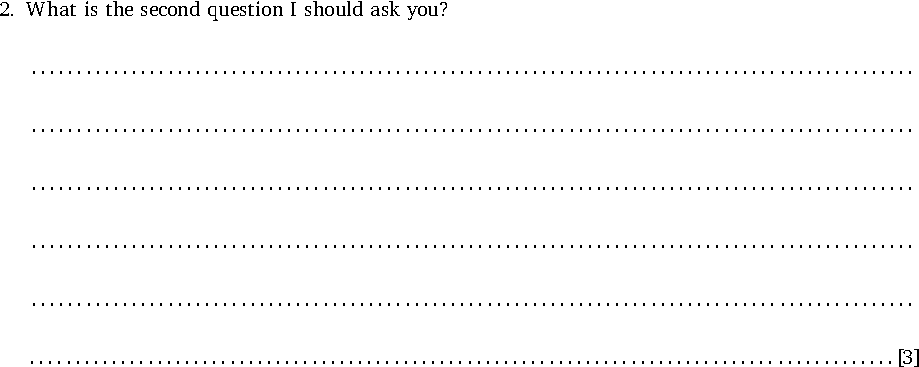
\includegraphics[width=0.7\textwidth]{imgs/drawing}
\end{center}
\pause

Code: 

\texttt{What is the second question I should ask you?}
$\backslash$\texttt{putansline\{6\}\{3\}}

\end{frame}

%----------------------------------------------------------
\begin{frame}[t] % 
\frametitle{Terminology}
\begin{itemize} 
  \item Document (the output) 
\item Document Class (the main type defining the doc) 
\item Package (a file encapsulating commands for a specific purpose) 
\item .sty (style files) 
\item .cls (document class files)
\item FNDB (filename database) 
\item update (… file/repository/meta information)  
\end{itemize}
\end{frame}


%----------------------------------------------------------
\begin{frame}[t] % 
\frametitle{Must See Documents}
\begin{itemize} 
  \item ``A Not So Short Introduction to LaTeX"
	\item ``The LaTeX Comprehensive Symbol List" 

\end{itemize}
\end{frame}
%----------------------------------------------------------
\begin{frame}[t] % 
\frametitle{Getting Started}
\begin{itemize} 
  \item To work with LaTeX, you need: 
  \begin{itemize}
 	 \item an editor ({\TeX}nicCenter, Kile, WinEdt, LED) 
  	 \item a compiler (Mik{\TeX}, {\TeX}Live, tetex ...)   
  \end{itemize}
  \item Enough talk. Let’s get started!
\end{itemize}
\end{frame}
%----------------------------------------------------------
\begin{frame}[t] % 
\frametitle{Demo}
\begin{itemize} 
  \item Installing software \pause
  \item Creating your first document \pause 
  \item Getting the required packages \pause 
  \item Creating your second document (an ACM format paper) \pause 
  \item Creating your third document (a Springer format paper) \pause
  \item Creating your fourth document (an IEEE transactions format paper) \pause   
  \item Algorithms \pause
  \item Mathematical typesetting \pause 
  \item Cool output boxes with line numbers!
 
\end{itemize}
\end{frame}
%----------------------------------------------------------
\begin{frame}[t] % 
\frametitle{Getting the Sources}
\begin{itemize} 
  \item You can get the resources for these sessions here:
  \url{http://www.csrdu.org/nauman/2011/10/16/latex-screencasts/} 
  \item Feel free to leave comments on the post there if you have any questions at all. I'll try to answer them as soon as possible. 
  \item All the required files (and completed documents) can be downloaded from this page. 
  \item You can find a really good resource on learning \LaTeX\ here: \url{http://ctan.org/tex-archive/info/lshort/english/lshort.pdf}
\end{itemize}
\end{frame}

\end{document}
